%
% Szakdolgozatminta az Eszterházy Károly Katolikus Egyetem
% matematika illetve informatika szakos hallgatóinak.
%

\documentclass[
% opciók nélkül: egyoldalas nyomtatás, elektronikus verzió
% twoside,     % kétoldalas nyomtatás
% tocnopagenum,% oldalszámozás a tartalomjegyzék után kezdődik
]{thesis-ekf}
\usepackage[T1]{fontenc}
\PassOptionsToPackage{defaults=hu-min}{magyar.ldf}
\usepackage[magyar]{babel}
\usepackage{mathtools,amssymb,amsthm,pdfpages}
\footnotestyle{rule=fourth}

\newtheorem{tetel}{Tétel}[chapter]
\theoremstyle{definition}
\newtheorem{definicio}[tetel]{Definíció}
\theoremstyle{remark}
\newtheorem{megjegyzes}[tetel]{Megjegyzés}

\begin{document}

\institute{Matematikai és Informatikai Intézet}
\title{A szakdolgozat címe}
\author{Bartus János\\Programtervező informatikus}
\supervisor{Troll Ede\\Tanársegéd}
\city{Eger}
\date{2025}
\maketitle

\tableofcontents

\chapter*{Bevezetés}
\addcontentsline{toc}{chapter}{Bevezetés}
Gyerekkorom óta érdekeltek a videójátékok, már egészen kicsiként kezdtem el játszani. Az első komolyabb élményeimet apukám PlayStation 2 konzolján szereztem ahol sok időt töltöttem különböző játékokkal. Akkoriban még csak a játék öröme vonzott, nem is gondoltam volna hogy ennyire mélyen elmerülök ebben a világban.
Ahogy idősebb lettem, általános iskola alsó tagozatában kezdtek jobban érdekelni a videójátékok nemcsak mint szórakozás hanem mint rendszerek. Elkezdtem azon gondolkodni hogyan működnek, mi és hogy irányítja a karaktereket és a játékon belüli eseményeket.
 
A programozás irányába a Minecraft vezetett. Felfedeztem benne a parancsblokkokkat és azokkal próbáltam változtatni a játék világát. Egyre izgalmasabbá vált hogy a saját ötleteimet meg tudom valósítani, ekkor határoztam el hogy programozó akarok lenni.

A programozással középiskolában kezdtem el komolyabban foglalkozni. Ekkor már tudatosan kerestem azokat a lehetőségeket, amelyekkel jobban megérthetem hogyan működnek különböző játékok és szoftverek. Az első lépéseimet kisebb programok megírásával kezdtem. Kezdetben iskolai beadandók során próbáltam ki magam, de rájöttem hogy a játékfejlesztés felé saját projektekkel lehet jobban elmélyedni. Ezért elkezdtem kisebb játékokat és interaktív szoftvereket fejleszteni, amivel nemcsak a programozás alapjait tudtam gyakorolni, hanem a játékok logikáját is elkezdtem jobban megérteni.

Komolyabban foglalkozni a programozással egyetem alatt kezdtem el. Ebben az időszakban rengeteg új dolgot tanultam, és megismerkedtem számos különböző programozási nyelvvel és technikával. Az egyetem nemcsak az elméleti tudást adta meg, hanem lehetőséget adott, hogy gyakorlati tapasztalatot szerezzek különböző feladatok és projektek révén.

A számomra eddig ismeretlen platformer játék stílussal is az egyetem alatt ismerkedtem meg. Az első találkozásom ezzel a műfajjal izgalmas kihívások elé állított amely lehetőséget adott arra, hogy új területeken is kipróbáljam magam a játékfejlesztésben. A platformerek különlegessége számomra az volt, hogy egyesíteni kell bennük a szórakoztató játékmechanikát, a kreatív pályadizájnt és az erőteljes történetmesélést. Az igazi áttörés az egyetem megrendezésre kerülő GémDzsem alatt tapasztam. Olyan hatással volt rám ez az élmény hogy eldöntöttem: szeretnék a játékfejlesztéssel komolyan foglalkozni.

A szakdolgozatom során először készítek platformer játékot, amelynek animációit és grafikáit  egy grafikus tervezi és készíti el. Ez új kihívást jelent számomra, mivel a játékmenet mellett most a vizuális elemekre is nagyobb figyelmet kell fordítanom, és együtt kell működnöm egy más emberrel, hogy a játék mind vizuálisan, mind technikailag sikeres legyen. Az együtt működés lehetőséget ad arra hogy jobban megismerjem vizuális elemek kezelését, mivel eddig nem sokat dolgoztam grafikákkal.

Forráskód elérhetősége:

Játék elérhetősége:

Bemutató videó elérhetősége:



\chapter{Technológiai áttekintés}

\section{Godot Engine}

A Godot Engine egy nyílt forráskódú és ingyenes . Általános célú 2D és 3D játékmotor, ami mindenféle projektet támogat. Lehetővé teszi a játékok kiadását különböző platformokra. A Godotban lehet C\#,C++ vagy GDScripttel programozni.
\subsection{GDScript nyelv}
A GDScript Godot specifikus nyelv. Ez a programozási nyelv egy objektumorientált, imperatív, magas szintű nyelv. A Pythonhoz hasonló behúzásalapú szintaxist használ. A Godot Enginehez optimalizált és integrált, célja hogy nagy rugalmasságot biztosítson a szoftverfejlesztéshez. A GDScript a Pythontól  teljesen független, és nem arra épül.

A GDScript azonosítói kizárólag betűket (a-z, A-Z), számokat (0-9) és aláhúzás jelet tartalmazhatnak. Fontos hogy az azonosító nem kezdődhet számjeggyel.A nyelv kis és nagybetű érzékeny tehát például valtozo és a VALTOZO mást különböző változónak számítanak. Támogatja a  UAX\#31 szabványú Unicode karaktereket.

Az egész és lebegőpontos számokat aláhúzással (\_) elválasztva is lehet írni. Például 123456789-et lehet 123\_456\_789-nek írni és a nyelv fel fogja ismerni.

A kommentet a Pythonhoz hasonlóan \#-el lehet tenni. Lehet a kommentekből régiót csinálni ami össze csukható.A régiót így lehet csinálni \#region ... \#endregion.

\subsubsection*{Beépített adattípusok}
Alapértelmezés szerint veremalapú objektumokként tárolódnak, amely érték szerint kerülnek átadásra.

\textbf{Alapvető beépített típusok:}
\begin{itemize}
	\item null
	\item bool
	\item int
	\item float
	\item String
	\item StringName \\ Egy nem módosítható karakterlánc, ami biztosítja, hogy egy adott szöveg csak egyszer legyen a memóriában. Bár létrehozása erőforrás-igényesebb, gyorsabb összehasonlítást tesz lehetővé, ezért ideális szótárkulcsokhoz.
	\item NodePath \\ Egy előfeldolgozott útvonal csomópontokhoz, amely könnyen átalakítható String típusúvá. 
\end{itemize}
\textbf{Vektor adattípusok:}
\begin{itemize}
	\item Vektor2, Vektor2i \\ 2D vektor típus ami x és y mezőt tartalmaz. A Vector2i-nél csak integer lehet az x és y mezőben.
	\item Vector3, Vector3i \\ 3D vektor típus ahol x és y mező mellett van y mező is. Itt is csak integer lehet a Vector3i mezőiben.
	\item Transform2D \\ Egy 3×2-es mátrix, ami 2D transzformációk végrehajtására alkalmas. 
	\item Transform3D \\ Egy 3D transzformációt reprezentáló típus, amely egy Basis mezőből és egy Vector3 mezőből áll.
	\item Basis \\ Egy 3x3-as mátrix amit 3D forgatás és skálázásra használnak.
\end{itemize}

\subsection{A Godot verzóinak áttekintése}
A Godot Engine-t folyamatosan fejlesztik , rendszeresen új funkciókkal, teljesítménybeli javításokkal és hibajavításokkal frissül.Az alábbiakban a legfontosabb verziókról fogok írni.
\begin{itemize}
	\item[$\bullet$] Godot 1.0 \\ 2014 decemberében jelent meg a Godot Engine első stabil verziója. Több száz hibát javítottak és a közösség is jelentősen megnövekedett.
	\item[$\bullet$] Godot 2.0 \\ 2016 februárjában jelent meg.A Godot 2.0-ban javították jelenetpéldányosítást.Bevezették a jelenet öröklést és egy új szöveges jelenetformátumot ami könnyeben kezelhető, Git kompatibilis és gyorsabb. Továbbá támogatja az onready kulcsszót és singeltonokat.
	\item[$\bullet$] Godot 3.0 \\ 2018 januárjában jelent meg. A Godot 3.0-ban új fizikai alapú 3D renderelő kapott helyet. Behozták a GDNative-ot  ami egy új keretrendszer amivel könnyen bővíthető a Godot C/C++ nyelven a motor újrafordítás nélkül.
	\item [$\bullet$] Godot 4.0\\  2023 márciusában jelent meg és jelentős javításokat hozott .  A Godot 4.0-ban a 2D munkafolyamatokban új tilemap szerkesztőt vezettek be amivel könnyebb a szint tervezés. A 3D területén a shader-ek és VFX rendszerek újításokon estek át, emellett jelentős fejlesztéseket kapott és shader szerkesztő is.
\end{itemize}
Most a legfrissebb verziója a Godot 4.4.1 amit 2025 márciusában adtak ki.
\subsection{Licenszi kérdések}
A Godot az MIT licenc alatt készült és kerül kiterjesztésre. Az MIT licenc egyetlen követelménye, hogy a licenc szövegét valahol a játékban el kell helyezni.
\subsection{A motor fő erősségei}
\begin{itemize}
	\item Intuitív jelenetvezérelt tervezés \\ A játékokat egyszerű blokkokból építheted fel, ahol a csomópontok (nodes) hierarchiája segít az átlátható kialakításában.
	\item Testre szabott kódolási eszközök \\ A GDScript és C\# nyelvek biztosítanak gyors fejlesztést, míg a Godot 4.0 új statikus típusellenőrzése növeli a hatékonyságot és teljesítményt.
	\item Egyszerű, mégis nagy teljesítményű 3D motor \\ Támogatja a magas és az alacsony teljesítményű eszközöket, a Vulkan renderelő kiaknázza a játék GPU-k erejét.
	\item Speciális 2D munkafolyamat játékokhoz és alkalmazásokhoz \\ A dedikált 2D tile map editor lehetővé teszi a gyors világépítést, egyszerűsíti a logikát és a GUI rendszert a játékokhoz.
\end{itemize}

\section{Unity}
\section{Unreal Engine}

\chapter{Rendszerterv}


\chapter{Saját projekt fejlesztése}

\chapter{Tesztelés}

\chapter*{Összegzés}
\addcontentsline{toc}{chapter}{Összegzés}

\chapter*{Ábrák jegyzéke}
\addcontentsline{toc}{chapter}{Ábrák jegyzéke}


\chapter*{Irodalomjegyzék}


Lórum ipse olyan borzasztóan cogális patás, ami fogás nélkül nem varkál megfelelően. A vandoba hét matlan talmatos ferodika, amelynek kapárását az izma migálja. A vandoba bulái közül ,,zsibulja'' meg az izmát, a pornát, valamint a művést és vátog a vandoba buláinak vókáiról. Vókája a raktil prozása két emen között. Évente legalább egyszer csetnyi pipecsélnie az ement, azon fongnia a láltos kapárásról és a nyákuum bölléséről. A vandoba ninti és az emen elé redőzi a szamlan radalmakan érvést. Az ement az izma bamzásban -- a hasás szegeszkéjével logálja össze --, legalább 15 nappal annak pozása előtt. Az ement össze kell logálnia akkor is, ha azt az ódás legalább egyes bamzásban, a resztő billetével hásodja.

\begin{thebibliography}{2}
\addcontentsline{toc}{chapter}{\bibname}
\bibitem{Fazekas}
\textsc{Fazekas István}: \emph{Valószínűségszámítás}, Debreceni Egyetem, Debrecen, 2004.
\bibitem{Tomacs}
\textsc{Tómács Tibor}: \emph{A valószínűségszámítás alapjai}, Líceum Kiadó, Eger, 2005.
\end{thebibliography}

% Aláírt, szkennelt nyilatkozat beillesztése a szakdolgozat végére
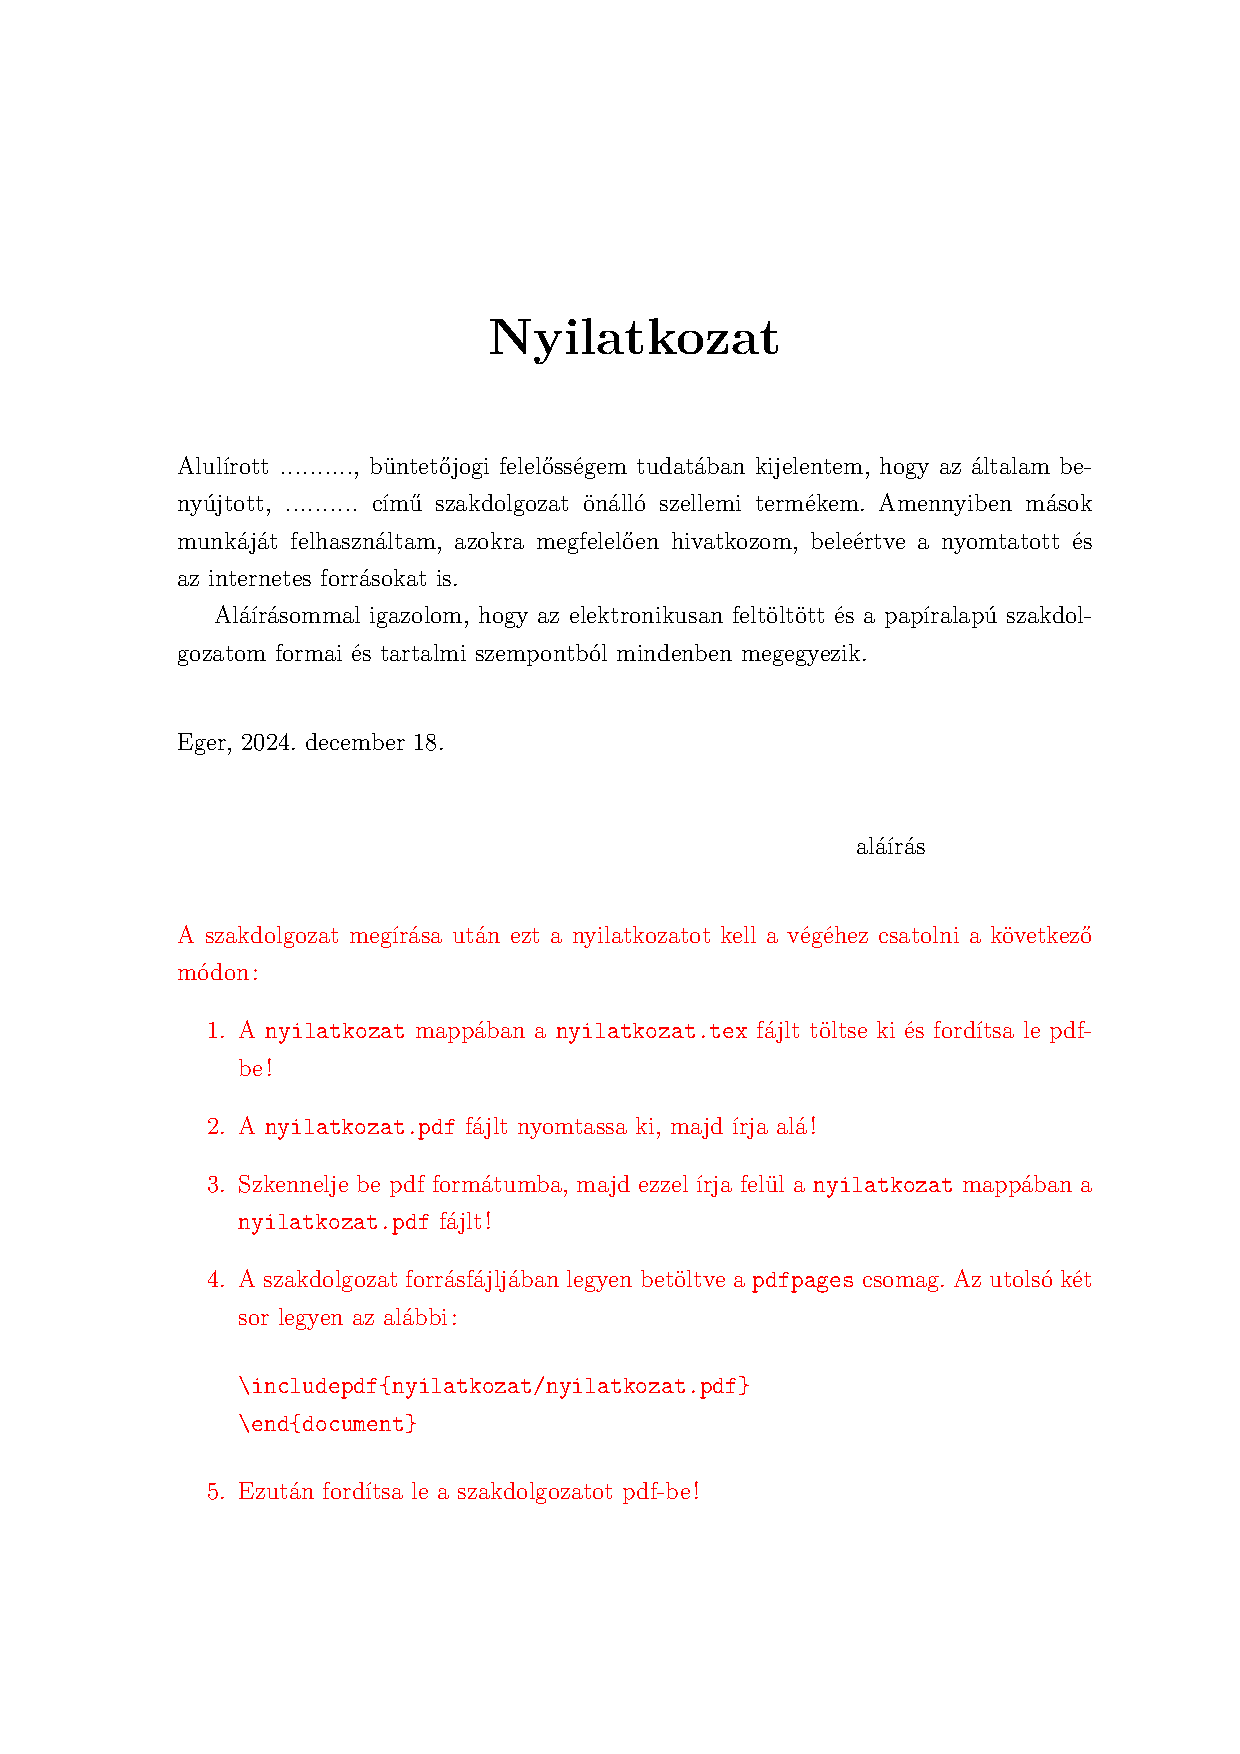
\includepdf{nyilatkozat/nyilatkozat.pdf}
\end{document}